\begin{figure}[tbp]
\centering
\begingroup
\newcommand{\geometrybandat}[5]{%
  \path[band#4] (#2,{#1-.20}) rectangle (#3,{#1+.20});
  \node[font=\scriptsize] at ({#5},#1) {$#4$};%
}
\newcommand{\geometryband}[4]{%
  \geometrybandat{#1}{#2}{#3}{#4}{(#2+#3)/2}%
}
\newcommand{\geometryrow}[2]{%
  \node[anchor=east,align=right,font=\scriptsize]
    at (-8.20,#1) {#2};%
}
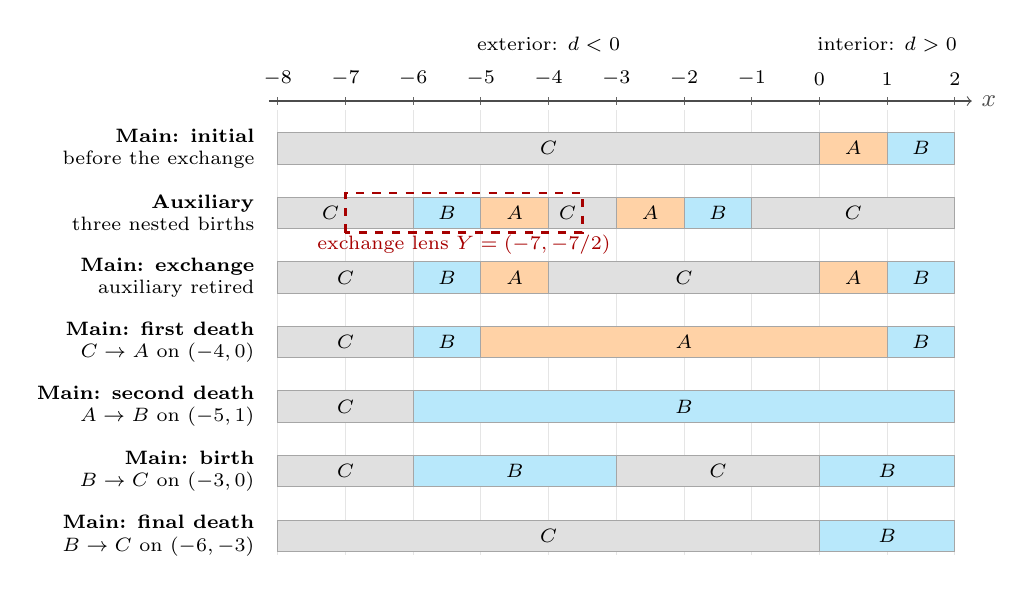
\begin{tikzpicture}[
  x=.86cm,y=1cm,
  bandA/.style={fill=orange!35,draw=black!35,line width=.3pt},
  bandB/.style={fill=cyan!28,draw=black!35,line width=.3pt},
  bandC/.style={fill=black!12,draw=black!35,line width=.3pt},
  lens/.style={draw=red!65!black,dashed,line width=.8pt}
]
  \foreach \geometrytick in {-8,-7,...,2} {
    \draw[black!10,line width=.3pt]
      (\geometrytick,.48) -- (\geometrytick,-5.17);
    \draw[black!60,line width=.35pt]
      (\geometrytick,.55) -- (\geometrytick,.65);
    \node[above,font=\scriptsize] at (\geometrytick,.67)
      {$\geometrytick$};
  }
  \draw[->,black!70] (-8.13,.60) -- (2.25,.60)
    node[right,font=\small] {$x$};
  \node[font=\scriptsize] at (-4,1.32) {exterior: $d<0$};
  \node[font=\scriptsize] at (1,1.32) {interior: $d>0$};

  \geometryrow{0}{\textbf{Main: initial}\\before the exchange}
  \geometryband{0}{-8}{0}{C}
  \geometryband{0}{0}{1}{A}
  \geometryband{0}{1}{2}{B}

  \geometryrow{-.82}{\textbf{Auxiliary}\\three nested births}
  \geometrybandat{-.82}{-8}{-6}{C}{-7.22}
  \geometryband{-.82}{-6}{-5}{B}
  \geometryband{-.82}{-5}{-4}{A}
  \geometrybandat{-.82}{-4}{-3}{C}{-3.72}
  \geometryband{-.82}{-3}{-2}{A}
  \geometryband{-.82}{-2}{-1}{B}
  \geometryband{-.82}{-1}{2}{C}
  \draw[lens] (-7,-1.07) rectangle (-3.5,-.57);
  \node[below,inner sep=0pt,font=\scriptsize,text=red!65!black] at (-5.25,-1.09)
    {exchange lens $Y=(-7,-7/2)$};

  \geometryrow{-1.64}{\textbf{Main: exchange}\\auxiliary retired}
  \geometryband{-1.64}{-8}{-6}{C}
  \geometryband{-1.64}{-6}{-5}{B}
  \geometryband{-1.64}{-5}{-4}{A}
  \geometryband{-1.64}{-4}{0}{C}
  \geometryband{-1.64}{0}{1}{A}
  \geometryband{-1.64}{1}{2}{B}

  \geometryrow{-2.46}{\textbf{Main: first death}\\$C\to A$ on $(-4,0)$}
  \geometryband{-2.46}{-8}{-6}{C}
  \geometryband{-2.46}{-6}{-5}{B}
  \geometryband{-2.46}{-5}{1}{A}
  \geometryband{-2.46}{1}{2}{B}

  \geometryrow{-3.28}{\textbf{Main: second death}\\$A\to B$ on $(-5,1)$}
  \geometryband{-3.28}{-8}{-6}{C}
  \geometryband{-3.28}{-6}{2}{B}

  \geometryrow{-4.10}{\textbf{Main: birth}\\$B\to C$ on $(-3,0)$}
  \geometryband{-4.10}{-8}{-6}{C}
  \geometryband{-4.10}{-6}{-3}{B}
  \geometryband{-4.10}{-3}{0}{C}
  \geometryband{-4.10}{0}{2}{B}

  \geometryrow{-4.92}{\textbf{Main: final death}\\$B\to C$ on $(-6,-3)$}
  \geometryband{-4.92}{-8}{0}{C}
  \geometryband{-4.92}{0}{2}{B}
\end{tikzpicture}
\endgroup
\caption{Normal-band words at one fixed $0<s<n$, in the coordinate
  $x=d/w(s)$ with $w(s)=10^{-3}\min(s,n-s)$; the chart displays only
  $-8\le x\le2$. The auxiliary starts uniformly at $C$ before the three
  nested births shown in its row. Exchanging the two sheets on the dashed
  lens creates the next main row: both displayed transverse boundaries
  lie in $C$ corridors on both sheets. The two deaths leave the interface
  at $x=-6$; the last
  birth and death move it to $x=0$, restoring the exterior label $C$.
  These are nominal labels: $A,B,C$ may coincide. This is a transverse
  schematic away from the edge endpoints and their point treatments.}
\label{fig:geometry-bands}
\end{figure}
